

\section{Natureza jurídica dos prestadores de serviços de saneamento nos municípios paulistas}\label{s2}


\begin{myexampleblock}{Quadro 1: Natureza jurídica dos prestadores de serviços de saneamento no estado de São Paulo}
   Administração Pública Direta $\rightarrow$ Prestação de serviços
públicos diretamente pelo próprio Estado. Seja ela da União, Estados e Municípios e Distrito Federal. \\
   
   Autarquia  $\rightarrow$ Entidade com personalidade jurídica de direito público, criada por lei específica, com patrimônio próprio, atribuições públicas
específicas e capacidade de auto administrar-se, sob controle estadual ou municipal. \\

Empresa pública $\rightarrow$ Entidade de personalidade jurídica de direito privado com patrimônio próprio e capital exclusivo da União, do Estado ou do
Município. Tem sua instituição autorizada por lei para prestação de serviço público passível de exploração econômica. \\

Empresa Privada $\rightarrow$ São as empresas que não estão ligadas ao Estado. \\

Sociedade de economia mista $\rightarrow$ Entidade de personalidade jurídica de direito privado com capital público e privado, maioria pública. 
\end{myexampleblock}




\begin{table}[H]\centering 
\begin{minipage}{0.8\textwidth}
  \caption{Natureza jurídica dos prestadores de serviços de abastecimento de água e esgoto dos municípios paulistas - 2019} 
  \label{tab:prop} 
\begin{tabular}{@{\extracolsep{5pt}} ccc} 
\\[-1.8ex]\hline 
\hline \\[-1.8ex] 
Natureza Jurídica & Número de municípios & Proporção de municípios \\ 
\hline \\[-1.8ex] 
	Adm. pública direta 	& $145$ 	& $22,48\%$ \\ 
	Autarquia 			& $88$ 	& $13,64\%$ \\ 
	Empresa privada 		& $23$ 	& $3,57\%$ \\ 
	Empresa pública 		& $2$ 	& $0,3\%$ \\ 
	Mista 				& $375$ & $58,14\%$ \\ 
    Sem Classificação	& $12$  & $1,86\%$ \\ 
\hline \\[-1.8ex] 
	Total               & 645    & $100\%$ \\
\hline \\[-1.8ex] 
\end{tabular} 
	\footnotesize \\
	Fonte: Elaborado pelos autores com dados do SNIS.
\end{minipage}
\end{table} 




\begin{figure}[H]
        \centering
        	\begin{minipage}{0.6\textwidth}	
                \caption{Distribuição espacial dos prestadores de serviços nos municípios paulistas}
                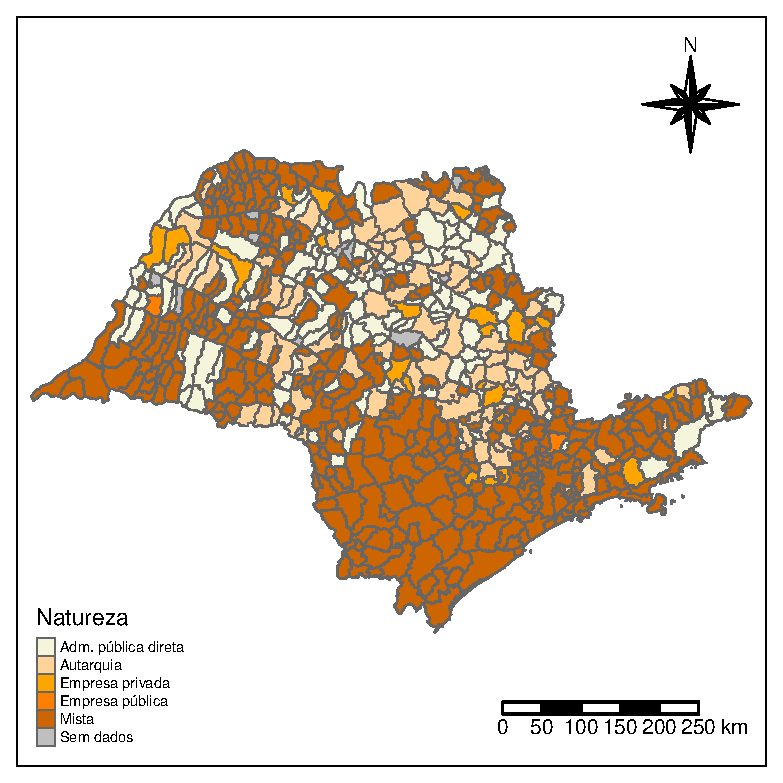
\includegraphics[scale=0.8]{figures/m1.eps}                 
            	\footnotesize \\
            		Fonte: Elaborado pelos autores com dados do SNIS.
    	\label{f:maps15}
	\end{minipage}
\end{figure}
